\subsection{package edu.kit.pse.fridget.client.datamodel}
\begin{figure}[H]
	       \centering
	       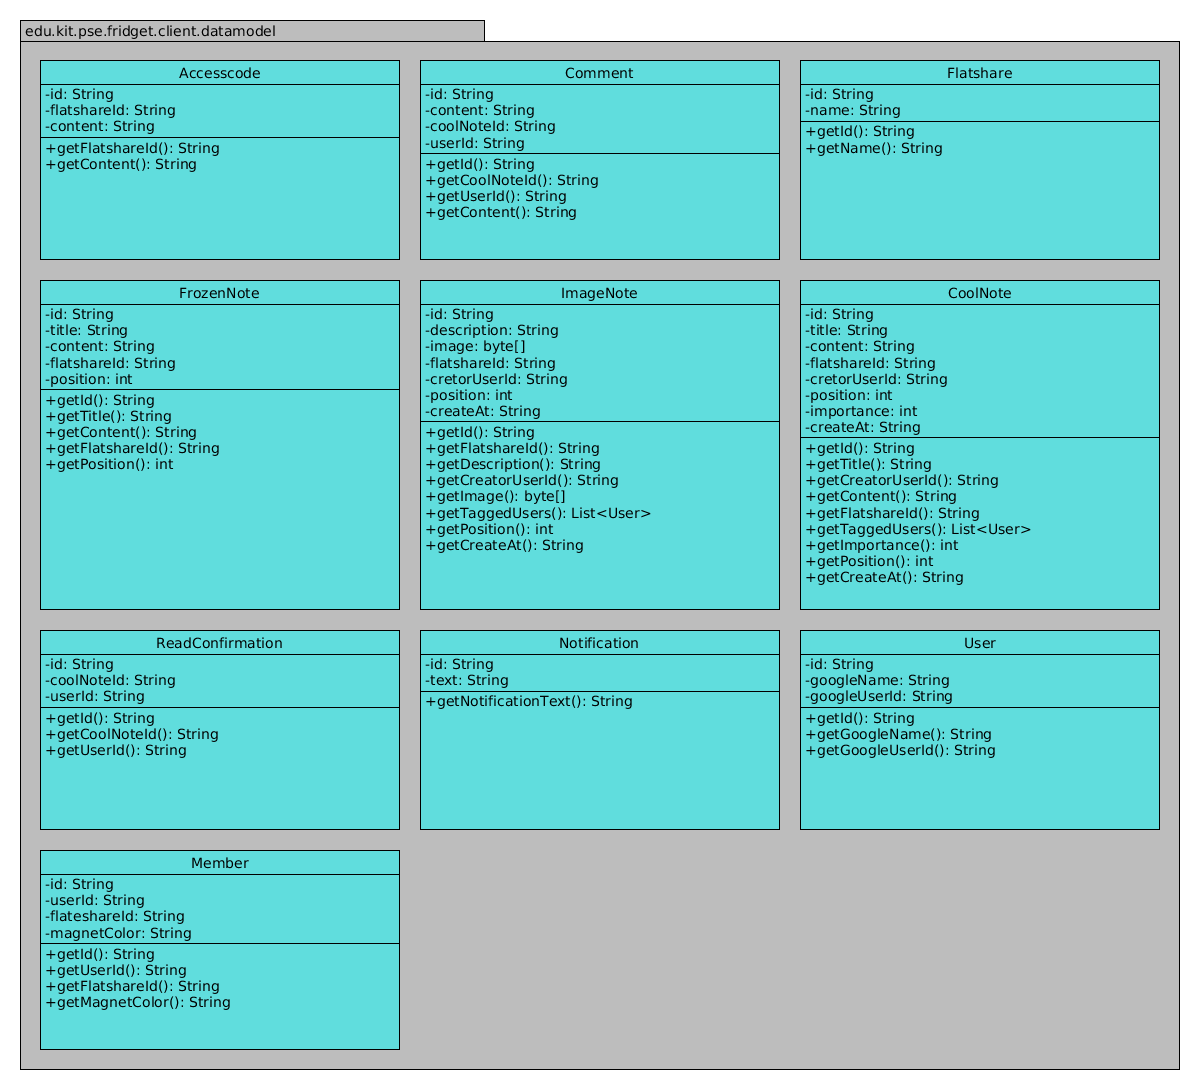
\includegraphics[scale = .35]{datamodel.png}
	       \caption{Klassen des Models}
	      \end{figure}
\subsubsection{\texttt{public class Accesscode}}

	\textbf{Beschreibung} \\
	\textit{Die Klasse Accesscode stellt der Access-Code, oder Zugangscode einer WG dar.} \\
	
	\textbf{Attribute}
	\begin{itemize}
		\item \textbf{id}: Die ID des Accesscode. \\
		\textbf{Typ:} String
		
		\item \textbf{flatshareId:} Die ID der WG zu der, die Accesscode gehört. \\
		\textbf{Typ:} String

		\item \textbf{content:} Der Inhalt der Accesscode.\\
		\textbf{Typ:} String
	\end{itemize}

	\textbf{Methoden}
	\begin{itemize}
		\item{\texttt{public String getFlatshareId()}}\\
		\textit{Gibt die ID der WG des Accesscodes zurück.}\\
		\item{\texttt{public String getContent()}}\\
		\textit{Gibt den Access-Code als String zurück.}\\
	\end{itemize}

	

\subsubsection{\texttt{public class User}}

	\textbf{Beschreibung} \\
	\textit{Die Klasse User stellt einen Benutzer der App dar.}\\
	
	\textbf{Attribute}
	\begin{itemize}
		\item \textbf{id:} Die ID des Benutzers. \\
		\textbf{Typ:} String
		\item \textbf{googleName:} Der Google-Name des Benutzers. \\
		\textbf{Typ:} String
		\item \textbf{googleUserId:} Die Google-ID des Benutzers. \\
		\textbf{Typ:} String
	\end{itemize}

	\textbf{Methoden}
	\begin{itemize}
	\item{\texttt{public String getId()}}\\
	\textit{Gibt die ID des Benutzers der App zurück.}\\
	\item{\texttt{public String getGoogleName()}}\\
	\textit{Gibt den Google-Namen des Benutzers zurück.}\\
	
	\item{\texttt{public String getGoogleUserId()}}\\
	\textit{Gibt die Google-ID des Benutzers der App zurück.}\\
	\end{itemize}

	

\subsubsection{\texttt{public class Member}}

	\textbf{Beschreibung} \\
	\textit{Die Klasse Member stellt einen Mitglieder einer WG dar.} \\
	
	\textbf{Attribute}
	\begin{itemize}
		\item \textbf{id:} Die ID des Mitgliedschafts. \\
		\textbf{Typ:} String
		\item \textbf{userId:} Die ID des Benutzers, der Mitglied eine WG ist. \\
		\textbf{Typ:} String
		\item \textbf{flatshareId}: Die ID der WG zu der, das Mitglied gehört. \\
		\textbf{Typ:} String
		\item \textbf{magnetColor:} Die Magnetfarbe des Mitglieds. \\
		\textbf{Typ:} String
	\end{itemize}

	\textbf{Methoden}
	\begin{itemize}
		\item\texttt{{public String getId()}}\\
		\textit{Gibt ID der Mitgliedschaft der Benutzer zur WG zurück.}\\
		
		\item\texttt{{public String getUserId()}}\\
		\textit{Gibt die ID des Benutzers der App, der Mitglied einer WG ist, zurück.}\\
		
		\item\texttt{{public String getFlatshareId()}}\\
		\textit{Gibt ID der Mitgliedschaft der Benutzer zur WG zurück.}\\
		
		\item\texttt{{public String getMagnetColor()}}\\
		\textit{Gibt die Magnetfarbe des Benutzers zurück.}\\
	\end{itemize}       

\subsubsection{\texttt{public class Flatshare}}

	\textbf{Beschreibung} \\
	\textit{Die Klasse Flatshare stellt eine WG dar, die in das App registriert ist.} \\
	
	\textbf{Attribute}
	\begin{itemize}
		\item \textbf{id:} Die ID der WG. \\
		\textbf{Typ:} String
		\item \textbf{name:} Der Name der WG. \\
		\textbf{Typ:} String
	\end{itemize}

	\textbf{Methoden}
	\begin{itemize}
		\item\texttt{{public String getId()}}\\
		\textit{Gibt die ID der WG zurück.}\\
		\item\texttt{{public String getName()}}\\
		\textit{Gibt den WG-Namen zurück.}\\
	\end{itemize}

\subsubsection{\texttt{public class CoolNote}}

	\textbf{Beschreibung} \\
	\textit{Die Klasse CoolNote stellt die Notiz der Art “Cool Note” dar, die aus einer Überschrift und schriftlichem Inhalt besteht. Cool Notes sind erstellbare, nicht editierbare, löschbare Notizen.} \\
	
	\textbf{Attribute}
	\begin{itemize}
		\item \textbf{id:} Die ID der Cool Note. \\
		\textbf{Typ:} String
		\item \textbf{title:} Die Überschrift der Cool Note. \\
		\textbf{Typ:} String
		\item \textbf{content:} Der Inhalt der Cool Note. \\
		\textbf{Typ:} String
		\item \textbf{flatshareId:} Die ID der WG, zu der die Cool Note gehört. \\
		\textbf{Typ:} String
		\item \textbf{creatorUserId:} Die ID der Benutzer der die Cool Note erstellt hat. \\
		\textbf{Typ:} String
		\item \textbf{position:} Die Position der Cool Note. \\
		\textbf{Typ:} int
		\item \textbf{importance:} Die Wichtigkeit der Cool Note. \\
		\textbf{Typ:} int
		\item \textbf{createAt:} Das Erstelldatum der Cool Note.\\
		\textbf{Typ:} String
	\end{itemize}

	\textbf{Methoden}
	\begin{itemize}
		\item\texttt{{public String getId()}}\\
		\textit{Gibt die Cool-Note-ID zurück.}\\
		
		\item\texttt{{public String getTitle()}}\\
		\textit{Gibt die Überschrift einer Cool Note zurück.}\\
		
		\item\texttt{{public String getCreatorUserId()}}\\
		\textit{Gibt die ID des Mitglieders zurück, der die Cool Note erstellt hat.}\\
		
		\item\texttt{{public String getContent()}}\\
		\textit{Gibt den Inhalt der Cool Note zurück.}\\
		
		\item\texttt{{public String getFlatshareId()}}\\
		\textit{Gibt die ID der WG zurück, zu der diese Cool Note gehört.}\\
		
		\item\texttt{{public List<User> getTaggedUsers()}}\\
		\textit{Gibt die Mitglieder zurück, die in der Cool Note getaggt sind. Wenn keine spezifiziert ist, sind alle Mitglieder der WG getaggt.}\\
		
		\item\texttt{public int getImportance()}\\
		\textit{Gibt die Wichtigkeit der Cool Note zurück.}\\
		
		\item\texttt{{public int getPosition()}}\\
		\textit{Gibt die Position der Cool Note zurück.}\\
		
		\item\texttt{{public String getCreateAt()}}\\
		\textit{Gibt das Erstelldatum der Image Note zurück.}\\
	\end{itemize}

\subsubsection{\texttt{public class FrozenNote}}

	\textbf{Beschreibung} \\
	\textit{Die Klasse FrozenNote stellt die Notiz der Art “Frozen Note” dar, die aus einer Überschrift und schriftlichem Inhalt besteht. Frozen Notes sind feste, editierbare, nicht löschbare Notizen.} \\
	
	\textbf{Attribute}
	\begin{itemize}
		\item \textbf{id:} Die ID der Frozen Note. \\
		\textbf{Typ:} String
		\item \textbf{title:} Die Überschrift der Frozen Note. \\
		\textbf{Typ:} String
		\item \textbf{content:} Der Inhalt der Frozen Note. \\
		\textbf{Typ:} String
		\item \textbf{flatshareId:} Die ID der WG, zu der die Frozen Note gehört. \\
		\textbf{Typ:} String
		\item \textbf{position:} Position der Frozen Note, die schon fest ist beim Erstellen der Pinnwand.\\
		\textbf{Typ:} int
	\end{itemize}
	
	\textbf{Methoden}
	\begin{itemize}
		\item\texttt{{public String getId()}}\\
		\textit{Gibt die Frozen-Note-ID zurück.}\\
		
		\item\texttt{{public String getTitle()}}\\
		\textit{Gibt die Überschrift einer Frozen Note zurück.}\\
		
		\item\texttt{{public String getContent()}}\\
		\textit{Gibt den Inhalt der Frozen Note zurück.}\\
		
		\item\texttt{{public String getFlatshareId()}}\\
		\textit{Gibt die ID der WG zurück, zu der diese Frozen Note gehört.}\\
		
		\item\texttt{{public int getPosition()}}\\
		\textit{Gibt die Position der Frozen Note zurück.}\\
	\end{itemize}

\subsubsection{\texttt{public class Notification}}

	\textbf{Beschreibung} \\
	\textit{Die Klasse Notification stellt die Benachrichtigung an den Benutzer über eine neue Cool Note dar.} \\
	
	\textbf{Attribute}
	\begin{itemize}
		\item \textbf{notificationId:} Die ID der Benachrichtigung. \\
		\textbf{Typ:} String
		\item \textbf{text:} Der Inhalt der Benachrichtigung. \\
		\textbf{Typ:} String
	\end{itemize}
	
	\textbf{Methoden}
	\begin{itemize}
		\item\texttt{{public String getNotificationText()}}\\
		\textit{Gibt den Benachrichtigungstext zurück.}\\
	\end{itemize}

\subsubsection{\texttt{public class Comment}}

	\textbf{Beschreibung} \\
	\textit{Die Klasse Comment stellt einen Kommentar dar, der unter der Cool Note geschrieben werden kann.} \\
	
	\textbf{Attribute}
	\begin{itemize}
		\item \textbf{id:} Die ID des Kommentars. \\
		\textbf{Typ:} String
		\item \textbf{content:} Der Inhalt des Kommentars. \\
		\textbf{Typ:} String
		\item \textbf{coolNoteId:} Die ID der Cool Note, zu der der Kommentar gehört. \\
		\textbf{Typ:} String
		\item \textbf{userId:} Die ID des Benutzers, der den Kommentar geschrieben hat.\\
		\textbf{Typ:} String
	\end{itemize}
	
	\textbf{Methoden}
	\begin{itemize}
		\item\texttt{public String getId()}\\
		\textit{Gibt die Kommentar-ID zurück}\\
		
		\item\texttt{{public String getUserID()}}\\
		\textit{Gibt die MemberID des Mitglieders zurück, der den Kommentar geschrieben hat.}\\
		
		\item\texttt{{public String getCoolNoteId()}}\\
		\textit{Gibt die CoolNoteID zurück.}\\
		
		\item\texttt{{public String getContent()}}\\
		\textit{Gibt den Inhalt des Kommentares zurück.}\\
	\end{itemize}

\subsubsection{\texttt{public class ImageNote}}

	\textbf{Beschreibung} \\
	\textit{Die Klasse ImageNote stellt die Notiz der Art “Cool Note” dar, die aus einer Überschrift und Bild besteht. Image Notes sind wie Cool Notes erstellbar, nicht editierbar und löschbar.} \\
	
	\textbf{Attribute}
	\begin{itemize}
		\item \textbf{imageNoteId:} Die ID der Image Note. \\
		\textbf{Typ:} String
		\item \textbf{description:} Die Beschreibung der Image Note. \\
		\textbf{Typ:} String
		\item \textbf{image:} Der Inhalt der Image Note. \\
		\textbf{Typ:} byte[]
		\item \textbf{flatshareId:} Die ID der WG, zu der die Image Note gehört. \\
		\textbf{Typ:} String
		\item \textbf{creatorUserId:} Die ID der Benutzer der die Image Note erstellt hat. \\
		\textbf{Typ:} String
		\item \textbf{position:} Die Position der Image Note. \\
		\textbf{Typ:} int
		\item \textbf{createAt:} Das Erstelldatum der Image Note.\\
		\textbf{Typ:} String
	\end{itemize}
	
	\textbf{Methoden}
	\begin{itemize}
		\item\texttt{{public String getID()}}\\
		\textit{Gibt die Image-Note-ID zurück.}\\
		
		\item\texttt{{public String getFlatshareId()}}\\
		\textit{Gibt die ID der WG zurück, zu der die Image Note gehört}\\
		
		\item\texttt{{public String getDescription()}}\\
		\textit{Gibt die Beschreibung einer Image Note zurück.}\\
		
		\item\texttt{{public String getCreatorUserId()}}\\
		\textit{Gibt die ID des Mitglieders zurück, der die Image Note erstellt hat.}\\
		
		\item\texttt{{public byte[] getImage()}}\\
		\textit{Gibt den Inhalt, also das Bild der Image Note zurück.}\\
		
		\item\texttt{{public List<User> getTaggedUsers()}}\\
		\textit{Gibt die Mitglieder zurück, die in der Image Note getaggt sind. Wenn keine spezifiziert ist, sind alle Mitglieder der WG getaggt.}\\
		
		\item\texttt{{public int getPosition()}}\\
		\textit{Gibt die Position der Image Note zurück.}\\
		
		\item\texttt{{public String getCreateAt()}}\\
		\textit{Gibt das Erstelldatum der Image Note zurück.}\\
	\end{itemize}

\subsubsection{\texttt{public class ReadConfirmation}}

	\textbf{Beschreibung} \\
	\textit{Die Klasse ReadConfirmation stellt die Check-Box dar, das dem Benutzer ermöglicht, für sich selbst sichtbar zu machen, ob der Benutzer eine Cool Note gelesen hat.} \\
	
	\textbf{Attribute}
	\begin{itemize}
		\item \textbf{readConfirmationId:} Die ID der Check-Box. \\
		\textbf{Typ:} String
		\item \textbf{coolNoteId:} Die ID der Cool Note, die als gelesen oder ungelesen markiert wird. \\
		\textbf{Typ:} String
		\item \textbf{userId:} Die ID der Benutzer der die Check-Box benutzt. \\
		\textbf{Typ:} String
	\end{itemize}
	
	\textbf{Methoden}
	\begin{itemize}
		\item\texttt{{public String getId()}}\\
		\textit{Gibt die Read-Confirmation- oder Lesebestätigung-ID zurück.}\\
		
		\item\texttt{{public String getUserId()}}\\
		\textit{Gibt die ID des Mitglieders zurück, der die Check-Box benutzt.}\\
		
		\item\texttt{{public String getCoolNoteId()}}\\
		\textit{Gibt die CoolNoteID zurück, die als gelesen oder ungelesen markiert wird.}\\
	\end{itemize}
